\begin{frame}{A Very Brief History of The Carpentries}
	\begin{columns}[T]
		\begin{column}[c]{.5\textwidth}
			\begin{itemize}
				\item It all started with this guy -->
				\item ... in 1998
			\end{itemize}
		\end{column}

		\begin{column}[c]{.5\textwidth}
			\begin{figure}
				\centering
				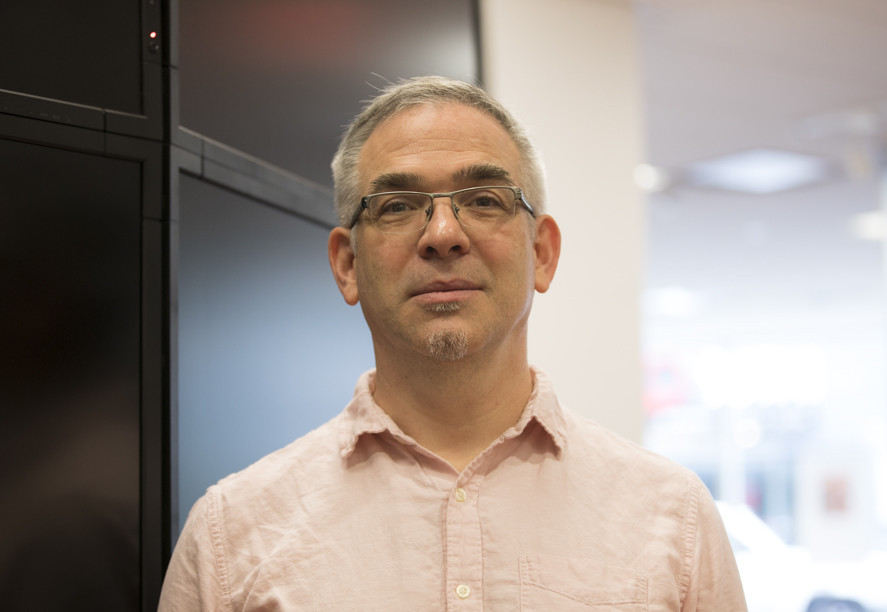
\includegraphics[width=.9\textwidth]{images/dr_greg_wilson.jpg} \linebreak
				\caption*{Dr Greg Wilson\linebreak\tiny\url{https://carleton.ca/scs/?p=14196}}
			\end{figure}
		\end{column}
	\end{columns}
	
	\note{It all started back in 1998 with Greg Wilson. I was watching a YouTube video of a talk he gave in 2014 at PyCon. And I don't think I could summarise it better than this quote from that talk}
\end{frame}

\begin{frame}{This is what Greg said about Software Carpentry}
	\begin{alertblock}{}
		\textbf{We are lab skills for scientific computing}. This project started because I was working with physicists and astronomers using first generation and parallel computers. And they would come into my office with their 50,000 lines of Fortran and ask me to make it a zillion times faster. And they had never heard of version control and weren't really sure why they should be writing functions because nobody every taught them. And it is unfair to look down on people if they are not doing things right if you have never shown them how.
		\linebreak
		
		\tiny\url{https://www.youtube.com/watch?v=FtKO619O5g0}
	\end{alertblock}

	\note[item]{We are lab skills for scientific computing}
	\note[item]{This project started because I was working with physicists and astronomers using first generation and parallel computers. And they would come into my office with their 50,000 lines of Fortran and ask me to make it a zillion times faster. And they had never heard of version control and weren't really sure why they should be writing functions because nobody every taught them. And it is unfair to look down on people if they are not doing things right if you have never shown them how.}
\end{frame}